\documentclass{article}\usepackage[]{graphicx}\usepackage[]{color}
%% maxwidth is the original width if it is less than linewidth
%% otherwise use linewidth (to make sure the graphics do not exceed the margin)
\makeatletter
\def\maxwidth{ %
  \ifdim\Gin@nat@width>\linewidth
    \linewidth
  \else
    \Gin@nat@width
  \fi
}
\makeatother

\definecolor{fgcolor}{rgb}{0.345, 0.345, 0.345}
\newcommand{\hlnum}[1]{\textcolor[rgb]{0.686,0.059,0.569}{#1}}%
\newcommand{\hlstr}[1]{\textcolor[rgb]{0.192,0.494,0.8}{#1}}%
\newcommand{\hlcom}[1]{\textcolor[rgb]{0.678,0.584,0.686}{\textit{#1}}}%
\newcommand{\hlopt}[1]{\textcolor[rgb]{0,0,0}{#1}}%
\newcommand{\hlstd}[1]{\textcolor[rgb]{0.345,0.345,0.345}{#1}}%
\newcommand{\hlkwa}[1]{\textcolor[rgb]{0.161,0.373,0.58}{\textbf{#1}}}%
\newcommand{\hlkwb}[1]{\textcolor[rgb]{0.69,0.353,0.396}{#1}}%
\newcommand{\hlkwc}[1]{\textcolor[rgb]{0.333,0.667,0.333}{#1}}%
\newcommand{\hlkwd}[1]{\textcolor[rgb]{0.737,0.353,0.396}{\textbf{#1}}}%

\usepackage{framed}
\makeatletter
\newenvironment{kframe}{%
 \def\at@end@of@kframe{}%
 \ifinner\ifhmode%
  \def\at@end@of@kframe{\end{minipage}}%
  \begin{minipage}{\columnwidth}%
 \fi\fi%
 \def\FrameCommand##1{\hskip\@totalleftmargin \hskip-\fboxsep
 \colorbox{shadecolor}{##1}\hskip-\fboxsep
     % There is no \\@totalrightmargin, so:
     \hskip-\linewidth \hskip-\@totalleftmargin \hskip\columnwidth}%
 \MakeFramed {\advance\hsize-\width
   \@totalleftmargin\z@ \linewidth\hsize
   \@setminipage}}%
 {\par\unskip\endMakeFramed%
 \at@end@of@kframe}
\makeatother

\definecolor{shadecolor}{rgb}{.97, .97, .97}
\definecolor{messagecolor}{rgb}{0, 0, 0}
\definecolor{warningcolor}{rgb}{1, 0, 1}
\definecolor{errorcolor}{rgb}{1, 0, 0}
\newenvironment{knitrout}{}{} % an empty environment to be redefined in TeX

\usepackage{alltt}
\IfFileExists{upquote.sty}{\usepackage{upquote}}{}
\begin{document}


\title {United States School Statistics: Chicago, Illinois
\\ IT497 OSEMN Assignment}
\author { Sonali Changkakoti
\\ School of Information Technology 
\\ Illinois State University
\\
\texttt{schangk@ilstu.edu}}
\date{\today} 
\maketitle


\section{Introduction}
Schools in the United States comprise of both public as well as private schools. The funding and control of public schools are done by state, local and federal government. Their curricula and staffing are decided by the locally elected school boards. On the other hand, private schools are generally free to determine their own curricula and staffing policies. There are also charter schools, which receive public funding but operate independently. Some states do not have charter school authorization. Around 88\% of school-aged students attend public schools, 9\% attend private schools and rest 3\% are homeschooled. 
\\Education in the United States is compulsory over an age range, which varies from state to state.  Formal education is divided into a number of stages. Schools are divided into three groups- elementary school, middle or junior high school and high school. The elementary school are from kindergarten to fifth grade, middle school are from 6th grade to 8th grade and high school are from 9th grade to 12th grade.Children may begin with pre-kindergarten, kindergarten or first grade. The compulsory education is till 12th grade, after that students can pursue higher education in colleges or universities.  
\\The data are collected from the National Center for Education Statistics for the number of schools, students, and teachers in regular schools with membership for the 100 largest cities in the United States, by school operational and charter status and state for school years ending 2001 through 2011. Here, the data from Chicago, IL among the 100 largest cities in the United States has been chosen for analysis.


\section {Data}
The data is collected for examining the total numbers of schools, teachers and schools in Chicago, IL over the period of 10 years, from December, 2011 to December, 2011. The required data is reteived from the Quandl API. Libraries like knitr, ggplot2 and reshape2 are used.

\begin{enumerate}
    \item Obtaing the data

The dataset is downloaded by using the Quandl API and auth token in a csv format.
It can be also access through the URL 
\\\verb@(https//www.quandl.com/NCES/SCHOOLS_CITIES_CHICAGOILLINOIS)@
The data is stored in myData object and it will be used for further analysis.
\begin{knitrout}
\definecolor{shadecolor}{rgb}{0.969, 0.969, 0.969}\color{fgcolor}\begin{kframe}
\begin{alltt}
\hlcom{# Loading knitr and Quandl}
\hlkwd{library}\hlstd{(knitr)}
\hlkwd{library}\hlstd{(Quandl)}

\hlcom{# To download data from a secure URL using Quandl API }
\hlcom{# and authcode}

\hlstd{myData} \hlkwb{<-} \hlkwd{Quandl}\hlstd{(}\hlstr{"NCES/SCHOOLS_CITIES_CHICAGOILLINOIS"}\hlstd{,}
                 \hlkwc{authcode}\hlstd{=}\hlstr{"sUMBj-Lb7MRzwnUWXvxe"}\hlstd{)}
\end{alltt}
\end{kframe}
\end{knitrout}
\item Scrubing data (Cleaning data)
 
Scrubing and cleaning of the data is done to get only the relevant data needed to obtain the results. Irrelevant data make the analyis difficult. Relevant data can be obtained by just looking into it and determining the requirements of the report. All the rows containing column 1 through column 4 are chosen and stored in a new object named cleanData.

\begin{knitrout}
\definecolor{shadecolor}{rgb}{0.969, 0.969, 0.969}\color{fgcolor}\begin{kframe}
\begin{alltt}
\hlcom{# Cleaning the data needed to plot a graph showing total }
\hlcom{# students, total teachers and total schools in Chicago, }
\hlcom{# Illinois}
\hlstd{cleanData}\hlkwb{<-}\hlstd{myData[,}\hlnum{1}\hlopt{:}\hlnum{4}\hlstd{]}
\end{alltt}
\end{kframe}
\end{knitrout}
The columns' name are also changed for convenience and readability. The cleaned data is shown as below:


\begin{knitrout}
\definecolor{shadecolor}{rgb}{0.969, 0.969, 0.969}\color{fgcolor}\begin{kframe}
\begin{alltt}
\hlcom{# Changing the columns' name}
\hlkwd{colnames}\hlstd{(cleanData)} \hlkwb{<-} \hlkwd{c}\hlstd{(}\hlstr{"year"}\hlstd{,} \hlstr{"schools"}\hlstd{,} \hlstr{"students"}\hlstd{,}
                         \hlstr{"teachers"}\hlstd{)}
\hlcom{# Showing the contents of cleanData}
\hlstd{cleanData}
\end{alltt}
\begin{verbatim}
##          year schools students teachers
## 1  2011-12-31     620   400383 21847.46
## 2  2010-12-31     614   402951 22588.93
## 3  2009-12-31     610   420193 21062.10
## 4  2008-12-31     600   399013 19674.00
## 5  2007-12-31     597   408311 18715.00
## 6  2006-12-31     600   415293 24659.00
## 7  2005-12-31     588   420787 23417.50
## 8  2004-12-31     588   428221 21261.90
## 9  2003-12-31     581   432478 22876.80
## 10 2002-12-31     574   432027 22419.10
## 11 2001-12-31     573   429684 23012.00
\end{verbatim}
\end{kframe}
\end{knitrout}
\item Explore data

The data is explored by using three functions - class(), str(), summary().
The function class prints the vector of names of classes an object inherits from.

\begin{knitrout}
\definecolor{shadecolor}{rgb}{0.969, 0.969, 0.969}\color{fgcolor}\begin{kframe}
\begin{alltt}
\hlcom{# Class function}
\hlkwd{class}\hlstd{(cleanData)}
\end{alltt}
\begin{verbatim}
## [1] "data.frame"
\end{verbatim}
\end{kframe}
\end{knitrout}
The function str compactly displays the internal structure of an R object, a diagonistic function and an   alternative to summary.

\begin{knitrout}
\definecolor{shadecolor}{rgb}{0.969, 0.969, 0.969}\color{fgcolor}\begin{kframe}
\begin{alltt}
\hlcom{# Str function}
\hlkwd{str}\hlstd{(cleanData)}
\end{alltt}
\begin{verbatim}
## 'data.frame':	11 obs. of  4 variables:
##  $ year    : Date, format: "2011-12-31" "2010-12-31" ...
##  $ schools : num  620 614 610 600 597 600 588 588 581 574 ...
##  $ students: num  400383 402951 420193 399013 408311 ...
##  $ teachers: num  21847 22589 21062 19674 18715 ...
\end{verbatim}
\end{kframe}
\end{knitrout}
And the summary is a generic function to produce result summaries of the results of various model functions. It is especially helpful for seeing basic descriptive statistics for all of the variables in a data frame and also the variables’ types.

\begin{knitrout}
\definecolor{shadecolor}{rgb}{0.969, 0.969, 0.969}\color{fgcolor}\begin{kframe}
\begin{alltt}
\hlcom{# Summary function}
\hlkwd{summary}\hlstd{(cleanData)}
\end{alltt}
\begin{verbatim}
##       year               schools         students         teachers    
##  Min.   :2001-12-31   Min.   :573.0   Min.   :399013   Min.   :18715  
##  1st Qu.:2004-07-01   1st Qu.:584.5   1st Qu.:405631   1st Qu.:21162  
##  Median :2006-12-31   Median :597.0   Median :420193   Median :22419  
##  Mean   :2006-12-31   Mean   :595.0   Mean   :417213   Mean   :21958  
##  3rd Qu.:2009-07-01   3rd Qu.:605.0   3rd Qu.:428953   3rd Qu.:22944  
##  Max.   :2011-12-31   Max.   :620.0   Max.   :432478   Max.   :24659
\end{verbatim}
\end{kframe}
\end{knitrout}



\end {enumerate}

\section {Result}

The three variables- schools, students and teachers are plotted against year (X-axis) in a line graph from the data obtained using the ggplot2 package. The melt command is used to reshape the data from wide to long format. The year variable is not melted as it identify the dataset's subject.

\begin{knitrout}
\definecolor{shadecolor}{rgb}{0.969, 0.969, 0.969}\color{fgcolor}\begin{kframe}
\begin{alltt}
\hlcom{# Melting the data}
\hlkwd{library}\hlstd{(reshape2)}
\hlstd{moltenData} \hlkwb{<-} \hlkwd{melt}\hlstd{(cleanData,}\hlkwc{id.vars}\hlstd{=}\hlstr{"year"}\hlstd{)}
\hlcom{# Plotting the grapg using ggplot2}
\hlkwd{library}\hlstd{(ggplot2)}
\hlkwd{ggplot}\hlstd{(moltenData,} \hlkwd{aes}\hlstd{(}\hlkwd{as.Date}\hlstd{(year,}\hlstr{"%e %b %Y"}\hlstd{),value))}\hlopt{+}
    \hlkwd{geom_line}\hlstd{(}\hlkwd{aes}\hlstd{(}\hlkwc{color} \hlstd{= variable))}\hlopt{+}
    \hlkwd{geom_point}\hlstd{()}  \hlopt{+} \hlkwd{xlab}\hlstd{(}\hlstr{"Year"}\hlstd{)} \hlopt{+} \hlkwd{ylab}\hlstd{(}\hlstr{"Total Number"}\hlstd{)}\hlopt{+}
    \hlkwd{labs}\hlstd{(}\hlkwc{title} \hlstd{=} \hlstr{"Total schools, total students and total 
    teachers"}\hlstd{)}\hlopt{+}\hlkwd{theme_bw}\hlstd{()}
\end{alltt}
\end{kframe}
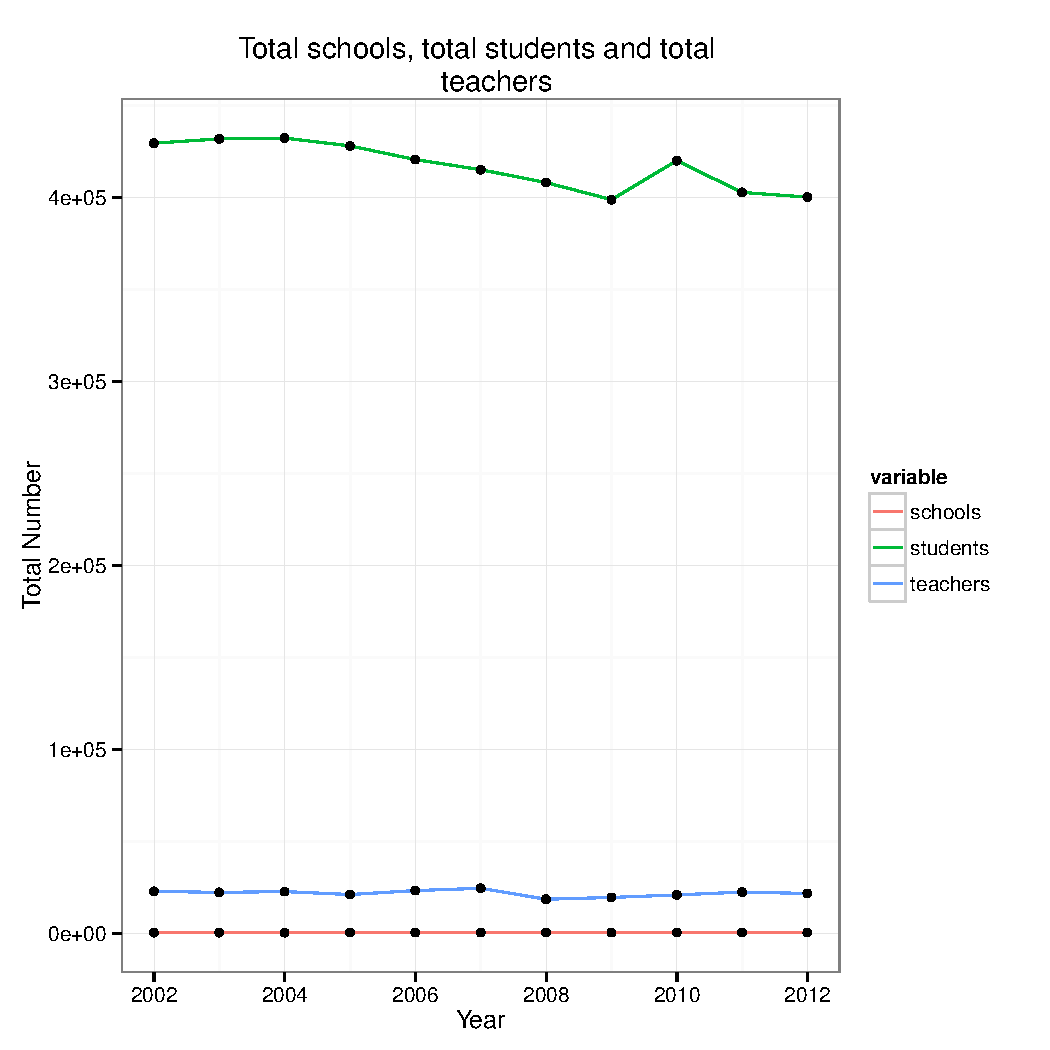
\includegraphics[width=\maxwidth]{figure/chunk7-1} 

\end{knitrout}
 
The graph has three different colored lines. The red,green and blue colored lines are of school, students and teachers variable, respectively. The total number of schools in 2001 was 573. It has some rise and fall in the total number. Finally, it became 620 in the year 2011.
\\The total number of students in 2001 was around 429,684, which decreased to around 399,013 in 2008. It again increased in 2009 to around 420,193 and finally decreased to 400,383 in 2011.
\\The total number of teachers in 2001 was 23,012, which reached its highest peak of around 24,659 in 2006. Later it decreased to around 18,715 in 2007. It again increased to around 22,589 in 2010 and finally fell to around 21,847 in 2011.
\end{document}
